%% ==============================
\chapter{Introduction}
\label{ch:introduction}
%% ==============================

\long\def\symbolfootnote[#1]#2{\begingroup%
\def\thefootnote{$*$}\footnote[#1]{#2}\endgroup} 

Graphs play an important role in modelling many types of systems or
relationships of data, such as
communication networks, evolutionary trees in biology or the friend
relationship in social networks. Moreover, graph drawings and especially
planar embeddings are important for layouting transistors on a VLSI-chip. For large graphs even the human aptitude for solving visual 
problems no longer suffices for determining drawings in reasonable time, and an
algorithmic approach on a computer has to be used.


A special drawing problem is \emph{$k$-page book embedding}, which was first introduced by Ollmann in 1973~\cite{Ollmann73}. It asks whether there is an embedding of a graph in a book with vertices along the book's \emph{spine} (a straight line) and 
edges in $k$~of the book's \emph{pages} (half~planes with the spine as boundary) such that the 
edges do not cross. The \emph{book thickness} of a graph~$G$ is the smallest~$k$ such
that~$G$ is $k$-page book embeddable. 

One application for book embedding is the automatic placement of components 
and the wiring between them on a multilayer printed circuit board. A wire may cross
layers but no two distinct wires may intersect in the same layer. The goal is then to find a good placement (we do not define what this actually means here).

%A wire may cross
%to another layer, but cannot intersect any other wire.
An approach to this problem, first introduced by So~\cite{So74}, is to arrange
the components on a regular grid and group elements together that should appear in the same
row or column. By introducing dummy elements, we\symbolfootnote[1]{Although this thesis has just one author, the first person plural is used instead of the singular. This should not be understood as pluralis maiestatis
but as an invitation to the reader to follow the thought processes of the author and is quite usual in mathematical
treatises.} can make sure that wires connect elements
in a single row or column. That is, we can layout the circuit board by layouting each
row and column individually. The variant of this single-row situation---introduced by Raghavan and Sahni~\cite{Raghavan83}---that does not allow wires to either cross a row or to change layers then directly corresponds
to a 2-page book embedding problem. This example was taken from a paper
by Chung et. al.~\cite{Chung87} that also provides several other practical
applications for book embedding, justifying the usefulness of the book embedding problem.

%We just cite one of their examples with a more %theoretical bent:
%\begin{quotation}
%One cancns
%\end{quotation}

In this thesis we consider a more restricted version of the book embedding problem where each edge
is assigned to the page is has to be embedded in, \ie we fix the \emph{page assignments}. In the remainder
of this chapter we formally define the book embedding problem (\myref{section:book-problem}), present related work (\myref{section:related}) and highlight the contribution of this thesis (\myref{section:contrib}).

\section{The Book Embedding Problem}\label{section:book-problem}

In this section we first present some basic definitions from graph theory. Then we formally formulate the problem \probBook that we consider in this thesis.

A \emph{graph} $G$ is a pair $(V, E)$ where $V$ is a non-empty finite set and
$E \subseteq \binom{V}{2}$. The set $V$ is called the set of \emph{vertices of~$G$}
and $E$ is the set of \emph{edges of~$G$}. We use $V(G)$ to refer to the vertices
of $G$~and $E(G)$ to refer to the edges of~$G$. A planar embedding of a graph~$G$ is a drawing of~$G$ in~$\SR^2$
such that edges do not intersect except at common endpoints. Planar embeddings are revisited more formally at the start of \myref{ch:preliminaries}.

A page embedding is a special planar embedding.

\begin{definition}
\label{def:page-embed}
A \emph{page embedding} of a graph $G = (V, E)$ is a planar embedding of~$G$ such that
the vertices of $G$ lie on the \emph{real line} $\SR \times \{0\}$ and every edge lies in the \emph{upper half-plane} $\bigl\{(x, y) \in \SR^2\colon y > 0\bigr\}$ apart from the edge's endpoints.
\end{definition}

\begin{figure}[\placement]
	\centering
	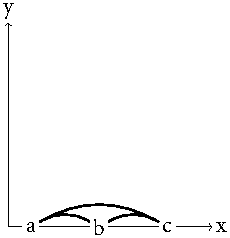
\includegraphics{figures/t_page_c3}
	\label{figure:page-c3}
	\caption[Page embedding of $C_3$]{A page embedding of $C_3$}
\end{figure}

\myref{figure:page-c3} depicts a page embedding for~$C_3$, the cycle on three~vertices.
By taking multiple page embeddings, we get a book embedding. 

\begin{definition}
\label{def:book-embed}
A \emph{book embedding} of graphs $G_1 = (V, E_1),\dotsc,\allowbreak G_k = (V, E_k)$ on the same set of vertices consists of page embeddings for each of the graphs that coincide in their vertex positions. 

In the setting of book embeddings the line $\SR \times \{0\}$
is also called the \emph{spine}. We only demand that edges in the same
graph~$G_i$ do not intersect. This can also be interpreted as giving each graph~$G_i$ its own upper half-plane, which we also call the \emph{page of~$G_i$}. Whenever we refer to a page in this thesis, we usually
mean the graph~$G_i$ on this page.
%The metaphor of an embedding into a book is then justified: The vertices are placed on the real line, the ``spine'' of the book, and the edges on their own copy of the upper half-plane, their ``page'' of the book. 
\end{definition}

The embeddability problem now asks whether such an embedding exists.
\newProb{\probBook}{A vertex set $V$ and edge sets $E_1,\dotsc, E_k \subseteq \binom{V}{2}$}
{Is there a book embedding of $(V, E_1),\dotsc, (V, E_k)$?}


In the literature \emph{book embedding} usually refers to the somewhat different problem \probBookNormal. Instead of directly embedding $k$~graphs
into $k$~pages, we first have to get $k$~graphs by arbitrarily partitioning the edges of a graph into 
$k$~parts and then embed these into $k$~pages. The problem
we call \emph{book embedding} is often called \emph{book embedding with fixed page assignment} in the literature. 
\newProb{\probBookNormal}{A vertex set $V$, an edge set~$E \in \binom{V}{2}$ and a number~$k\geq 1$}
{Is there a partition~$E = \bigcup_{i=1}^{k} E_i$ such that $(V, E_1), \dotsc, (V, E_k)$ is book embeddable?}
We depict this
assignment of the edges to the pages that has already been fixed either by using different colours or in the case of exactly two pages by one set of edges being drawn above and one below the spine.

\section{Related Work}
\label{section:related}

The \probBook problem is a graph drawing problem that is closely related to simultaneous planar drawings. Bläsius, Kobourov
and Rutter~\cite{GD2012} provide a good overview of those types of problems. 

In this section 
we first list some useful results about the usual book embedding problem \probBookNormal.
Then we present the literature about its variant \probBook.  
The fixed page problem \probBook had not been well-studied before the writing of this thesis. Thus, the list
of published results is quite small, even though it is exhaustive.

Furthermore, we introduce the concept of a \PQ-tree here, as first described by Booth and Lueker~\cite{Booth76}. Although \PQ-trees are not directly related to book embeddings,
we use them in many of the special cases in \myref{chapter:special}. Thus,
we also reference some results about \PQ-trees at the end of the section.

\begin{figure}[\placement]
    \centering
    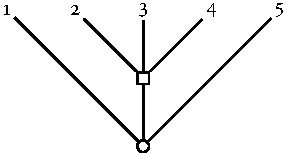
\includegraphics{figures/t_pq-tree}
    \caption[Simple \PQ-tree]{A simple \PQ-tree. \PT-nodes are drawn as a circle \tikz[scale=0.4,baseline={([yshift=+0.1em]current bounding box.south)}] \draw (0,0) circle (1em);, \Q-nodes as a box \tikz[scale=0.75,baseline={([yshift=+0.1em]current bounding box.south)}] \draw (-0.5em, -0.5em) -- ++(1em, 0) -- ++(0, 1em) -- ++ (-1em,0) -- cycle;.}
    \label{figure:pq}
\end{figure}

\begin{definition}\label{def:pq}
A \emph{\PQ-tree} $T$~on $M := \range{n}$ is a rooted, ordered
tree with leaves~$M$ and inner nodes either of type~$P$ 
or type~$Q$.

The tree represents a set of permutations $\pi(T) \subseteq \Sym(M)$ on its leaves as follows: The order of the children
of a \PT-node can be permuted in any way, while the order of the children of a \Q-node can only be reversed. The set~$\pi(T)$ then consists exactly of the permutations of the leaves~$M$ that we can get
by flipping the inner nodes in any of the specified valid ways.

The empty set of permutations on a set cannot normally be described by a \PQ-tree, so we define the	 special \emph{null tree} $\varepsilon$ representing~$\emptyset$.
Furthermore, let a \emph{\PT-tree} be a \PQ-tree containing only \PT-nodes as inner nodes and a \emph{\Q-tree} be a 
\PQ-tree only containing \Q-nodes as inner nodes.
\end{definition}

For example, the \PQ-tree in \myref{figure:pq} represents the permutations 12345, 14325, 52341, 54321, 15234,  15432,  51234,  51432, 23415, 43215, 23451 and 43251.

\paragraph{Book Embedding without Fixed Page Assignments}

We first enumerate some results for \probBookNormal. We do not use
these results, but they are still a helpful point of reference for classifying our
findings about the fixed page case \probBook.

There are a variety of results about small page numbers: The graphs
embeddable in a single page are just the outerplanar graphs and a graph
is embeddable into two pages if and only if it is \emph{sub-hamiltonian}, \ie a subgraph of a planar Hamiltonian
graph, as shown by Bernhart and Kainen~\cite{Bernhart79}. Widgerson~\cite{Widgerson82} proved
that checking a maximal planar graph for Hamiltonicity is \NP-complete, \ie \probBookNormal is already
\NP-complete if we restrict ourselves to two pages.

Thus, the book embedding problem for $k \ge 2$~pages is probably not efficiently solvable.
One viable research direction following this insight was to consider variations of the problem
or special graphs. Indeed, there are results for several graphs, including
but not limited to the following: A planar graph is embeddable into four pages~\cite{Yannakakis86},
a graph of treewidth~$k$ has book thickness at most~$k + 1$~\cite{Dujmovic07} and genus~$g$
graphs have book thickness~$\OO(\sqrt{g})$~\cite{Malitz88}. We do not explain these results further as we do not use them.

\paragraph{Book Embedding with Fixed Page Assignments}

In contrast, little is known about the variant \probBook with fixed page assignments. The only result we could find appears
in a recently published technical report by Hong and Nagamochi~\cite{two-page-09}. They show
that \probBook is decidable in linear time for two pages, unlike \probBookNormal. That is, the argument for the \NP-completeness of \probBookNormal
cannot be adopted for fixed page assignments. 

Furthermore, Angelini et.\,al.~\cite{angelini11} provide an interesting application for the
\probBook problem. They consider the important special case \SEFECON, whose complexity is unknown, of the simultaneous embedding problem \SEFE and reduce it to a 2-page \probBook problem where
the vertex order on the spine is additionally constrained by a \PT-tree.

\newProb{\SEFE}{Two graphs~$G_1$ and~$G_2$.}{Are there planar embeddings
of~$G_1$ and~$G_2$ that coincide on~$G_1 \cap G_2$?}
\newProb{\SEFECON\label{prob:sefecon}}{Two graphs~$G_1$ and~$G_2$ where~$G_1 \cap G_2$ is connected.}{Are there planar embeddings of~$G_1$ and~$G_2$ that coincide on~$G_1 \cap G_2$?}


\paragraph{PQ-trees}
The concept of a \PQ-tree was originally described by Booth and Lueker~\cite{Booth76} to solve
the consecutive ones problem: Given a 0-1-matrix, is there a permutation of its columns
such that the 1's in every row appear consecutively? Let~$T$ be a \PQ-tree and~$S$ some
subset of its leaves. Then they showed that there is an operation $\reduce(T, S)$, computable
in $\OO\bigl(|S|\bigr)$~time, that
yields a \PQ-tree representing exactly the permutations in~$\pi(T)$ where all leaves in~$S$ appear
consecutively. Thus, the consecutive ones problem can be solved by starting
with a \PQ-tree representing all permutations on the columns (a single \PT-node) and reducing on the columns containing~1's row by row. This reduction operation proves useful for solving the variations on
book embedding in \myref{chapter:special}. 

Booth~\cite{Booth75} additionally showed that we can intersect two \PQ-trees in linear
time, \ie from two \PQ-trees $T_1$ and $T_2$ on the same leaves we can construct a \PQ-tree representing~$\pi(T_1) \cap \pi(T_2)$ in linear time.

We also make use of the fact that there are linear time planarity algorithms that test a graph~$G$
for planarity and embed~$G$ vertex-by-vertex.
% such that at each have step and for each component of the
%already embedded graph we get a \PQ-tree that represents the possible orders of the half-embedded edges %in an
%extension of this partial embedding. 
The general scheme for these algorithms is summarised by Haeupler and Tarjan~\cite{Haeupler08}. 
Their scheme unifies and simplifies several similar linear-time planarity algorithms:
\begin{enumerate} 
\item The Lempel-Even-Cederbaum algorithm~\cite{Lempel67} that was refined
to run in linear time by Booth and Lueker~\cite{Booth76}
\item The Shih-Hsu algorithm~\cite{Shih93}
\item The Boyer-Myrvold algorithm~\cite{Boyer99}
\end{enumerate}

\section{Contribution and Outline}
\label{section:contrib}

From the literature analysis above we can see that there are a lot of open problems
for \probBook. For example: Is \probBook \NP-complete for a linear number
of pages? Does \probBook remain efficiently solvable for 3~pages? What happens when we constrain
the vertex orders by a \PQ-tree?

In this thesis we want to solve some of these open problems and provide points of reference for further
research. We first consider the time complexity of \probBook and then some special cases or restrictions thereof. More specifically, this work is structured as follows:

\begin{description}
\item[\myref{ch:preliminaries}] Firstly, we provide basic definitions and results
we need in the rest of the thesis. This is followed by rephrasing \probBook as a 
total ordering problem \probBookOrder. At the end of the chapter we begin to actually study book embeddings by identifying some of the freedoms we have in choosing total orders that solve an \probBookOrder instance. 
\item[\myref{chapter:complexity}] As alluded to above, in this chapter we show that the \probBook problem
is \NP-complete for an unbounded number of pages by reduction from the betweenness problem that is
also defined in this chapter. 
This result even applies if the edges on each page form a matching.

Since we still want to decide book embeddability for some graphs, we then show
how to solve \probBook in exponential time by expressing book embeddability using 3-\CNF-formulae. We also provide some optimisations for these formulae.
\item[\myref{chapter:special}] This chapter contains our main results. We discuss
and solve \probBook for several special cases and restrictions.

Firstly, we show that \probBook can be solved in linear time if each
page is a connected graph on all vertices. 

Then
we proceed with the opposite, the almost completely disconnected case, \ie we take disjoint perfect matchings as pages. We already
know that \probBook is \NP-complete for (general) matchings on the pages, at least if
we allow an unbounded number of pages. It is not clear whether perfect matchings make \probBook easier.

Still, we can give a necessary
criterion when the pages are perfect matchings, namely the union of all the pages has to be a bipartite graph. This criterion is not sufficient. Indeed, we then find both bipartite examples and counterexamples
for all numbers of pages, partly using computer assistance.

We continue with a variation on book embedding. Motivated by a result of Angelini et.\,al.~\cite{angelini11}, we consider book embeddings with the additional constraint that the
order of the vertices must be represented by a given \Q-tree. We show that this restricted case is
solvable in quadratic time.

The chapter closes with another variation on \probBook. We take multiple spines~(parallel lines)
in the plane and associate every vertex with a spine it has to be drawn on. 
Additionally, we impose the restriction that edges must be drawn between consecutive spines, above the
topmost spine or below the bottommost spine. Unlike the previous case, we do not solve this
variation. We just show that it is equivalent to
\probBook with 2~pages where the vertex order is constrained
by a special kind of \PT-tree. If we did not allow the edges to go
above the topmost or below the bottommost spine, this variation would be the same as the level planarity problem, which was first introduced by Tomii~et.~al.~\cite{Tomii77}. Jünger, Leipert and
Mutzel presented an algorithm that checks for level planarity in linear time~\cite{Junger99}.
\item[\myref{ch:conclusion}] The thesis is concluded by summarising the results
we obtained and discussing viable future research directions.
\end{description}

%This chapter should contain
%\begin{enumerate}
%  \item A short description of the thesis topic and its background.
%  \item An overview of related work in this field.
%  \item Contributions of the thesis.
%  \item Outline of the thesis.
%\end{enumerate}

%%% Local Variables: 
%%% mode: latex
%%% TeX-master: "thesis"
%%% End: 
